\documentclass[emulatestandardclasses]{scrartcl}
\usepackage{graphicx}
\usepackage{color}
\usepackage[ngerman]{babel}
\usepackage{hyperref}
\usepackage{fullpage}
\usepackage[utf8]{inputenc}
\usepackage{calc} 
\usepackage{enumitem}
\usepackage{titlesec}
\newcommand{\todo}[1]{\textcolor{red}{TODO: #1}\PackageWarning{TODO:}{#1!}}
\date{\vspace{-3ex}}
\begin{document}

\title{
	\includegraphics*[width=0.75\textwidth]{ErstesSem/images/hu_logo.png}\\
	\vspace{24pt}
	Die Erfahrung der Realität\\durch Widerstand}
\subtitle{\vspace{10pt}Proseminar WS 17/18\\
          Matthias Schlo"sberger\\
          Philosophisches Institut I \\ 
          Humboldt Universit"at zu Berlin}
\author{Lennard Wolf\\
        \small{\href{mailto:lennard.wolf@student.hu-berlin.de}{lennard.wolf@student.hu-berlin.de}}}
\maketitle
\begin{abstract}
Häufig wird Erkenntnistheorie als Versuch der Rechtfertigung von Erkenntnis betrieben. Dass es möglich ist, von der Rechtfertigung einer Erkenntnis zu sprechen, verweist auf ein Problem, das vor allen Fragen der Rechtfertigung geklärt werden sollte. Bevor eine Erkenntnis gerechtfertigt werden kann, muss das in der Erkenntnis Erkannte erfahren werden. Dies, so die Arbeitshypothese des Seminars, gilt auch und insbesondere für die Erfahrung von Realität.
Eine mögliche Antwort auf die Frage, wie die Erfahrung der Realität gemacht wird, lautet: durch die Erfahrung der Widerständigkeit von etwas (der Welt, des Psychischen, des Physischen, des Anderen etc.). Ziel des Seminars ist es, diese Antwort bei einigen für dieses Thema klassischen Autoren zu untersuchen. Besonders wichtig wird es sein, einen klaren Begriff des Widerstands zu entwickeln, der an vielen verschiedenen Phänomenen erläutert werden kann.

\end{abstract}
\newpage

\tableofcontents
%\listoffigures
\newpage


\section{Einf"uhrung\\(19.10.17)}

\begin{itemize}
  \item Moodle-Passwort: Scheler
\end{itemize}


\subsection{Überblick über die Fragestellung}

\begin{itemize}
  \item Realismus vs. Idealismus
  \item Fragestellungen dieser Alternative: Ob wir Zugang zu Realität/Wirklichkeit haben und wenn ja, welchen?
  \item Realisten: Ja.
  \item Idealisten: Die Wirklichkeit wie sie an sich ist können wir nicht erfahren, sondern: das was wir als Wirklichkeit erfahren das ist immer Konstruktion des Subjekts (\emph{subjektiver Idealismus}) oder durch kollektive Konstruktion (\emph{Konstruktivismus})
  \item Essenzaussagen oder Existenzaussagen (was vs. dass) sind gekoppelt an Idealismus vs. Realismus
  \item Matrix: was oder dass Problem
  \item Descartes Ausgangsfrage: Wir müssen alles in Zweifel ziehen. Was bleibt übrig: ego das cogito machen tut (\emph{cogito existo})
  \item Wie können wir von unserer Existenz auf die Existenz der Welt schließen?
  \item Ist die Welt geträumt? Wie unterscheiden wir Traum und Wirklichkeit?
  \item Um zu fragen, ob das Wirklichkeit ist, muss ich mit dem Gegenteil bekannt sein.
  \item Ob das Urteil darüber wahr ist, ist eine andere Frage. (erst danach!)
  \item Klassische Frage: Gibt es Beweise dafür, ob die sogenannte außenwelt existiert?
  \item Übersieht, dass anderer Frage vorgelagert ist: Wie können wir dazwischen unterscheiden?
  \item Philosophie als Fundierungsprojekt! Unterscheidungsfrage ist noch zu klären!
  \item Damit wird die Frage Realismus vs. Idealismus nicht überflüssig! (wie Scheler, Carnap behauptet haben)
  \item Aber: Ändert dieses Fundierungsprojekt überhaupt etwas an der Unterscheidung?
  \item Ob wir in Erfahrungen, durch die wir mit der Unterscheidung vertraut werden, ob das wahr ist, sei erstmal dahingestellt. (macht nichts wenn wir vertauschen, denn wir sind trotzdem mit der Unterscheidung bekannt!)
  \item Dildheim: Über den Grund zur Annahme zur Existenz der Außenwelt 
  \item Repräsentationalismus: Annahme: Zugang zur Welt ist, dass sie vorgestellt ist, dass die Welt in meinem Bewusstsein, dann bedarf es eines Kriteriums dafür, dass die echte Welt 
  \item Naiver, Direkter und Kritischer Realismus
  \item Derealisierung: Die anderen sind da, aber nicht wirklich
  \item Inwiefern können wir uns die ganzen Sinne vorstellen?
  \item Bedeutung der Frage: In welchen Akten unterscheiden wir die Wahrnehmung als wirklich und unwirklich?
  \item Ist das zu kurz gekommen weil wir in erkenntnistheoretischen Fragen uns nur Rechtfertigungen beschäftigt haben und weil wir uns zu sehr an dem "`visozentrischen"' Modell orientiert haben?
  \item \emph{In diesem Seminar Hauptclaim}: Tastsinn wurde eminent vernachlässigt, obwohl dieser zunächst von der Wirklichkeit der Welt überzeugt ist
  \item Aus diesem Widerstand ziehen wir die tiefe Überzeugung, dass die Welt da ist!
  \item Haben Leute mit Derealisierungsproblemen Schwierigkeiten mit dem Widerstand?
  \item Gründen alle Erfahrungen der Welt in Widerständen?
  \item Entfremdungsphänomene: Hier ist jemand nicht mehr in der Lage, Widerstandserfahrungen zu machen.
  \item Vernunfteinsichten helfen nicht weiter! Sie können Problem fixieren, aber nicht lösen.
\end{itemize}

\subsection{Gestaltung des Semesters I}

\begin{itemize}
  \item Erster Schritt: Platons Höhlengleichnis - vergegenwärtigen, was das Grundproblem von Realismus/Idealismus ist
  \item Zweiter Schritt: Text, der entscheidender Bezugspunkt Entwicklung des Widerstandsarguments Grund Über den Grund zur Annahme zur Existenz der Außenwelt
  \item Dritter Schritt: Scheler: Hat am schärftsten artikuliert (auch vllt. David Katz ("`Aufbau der Tastwelt"') zur Anregung)
  \item Letztes Drittel: Merleau-Ponty, Waldenfels (responsive Ethik), Psychopathologische Phänomene (Thomas Fuchs (Karls Jaspers Lehrstuhl in Heidelberg))	
\end{itemize}

\section{Platons Höhlengleichnis\\(26.10.17)}

\subsection{Lektürenotizen}

\begin{itemize}
  \item Zwei Dinge die der Befreite sieht: Die Schatten, und die schattenwerfenden Dinge
  \item Erst seit er beides kennt, ergibt sich die Frage, welches denn nun die Realität sei
  \item Durch Gewöhnung kommt er in Schmerzen dann zum Erkennen des Neuen
  \item Er wird sich an den Spielen und Hierarchien der alten Freunde nicht mehr erfreuen können, es wäre nicht mehr so echt wie früher. So würde er sich lieber versklaven lassen in der neuen Wahrheit als König sein im Falschen.
  \item Diese alten würden ihn auch nicht ernst nehmen
\end{itemize}

\subsubsection{Fragen}

\begin{itemize}
  \item Ist nicht gerade die Bewegung der Erkenntnis unsere Grundlage für die Unterscheidung? Das heißt, wenn das Wissen das erste Mal als kontrafaktisch erkannt wird, dann ergibt sich schon die Möglichkeit der Frage nach Realität..?
\end{itemize}

\subsection{Gestaltung des Seminars II}

\begin{itemize}
  \item Dilthey, Scheler: Basalster Zugang zur Welt: Widerstand
  \item Erkenntnistheorie der Sinne und ihrer kognitiven Leistungen
  \item David Katz, Wechselspiel mit Scheler, Gestaltpsychologie
  \item Gestaltpsychologe: Jede Wahrnehmung ist eine Wahrnehmung eines Ganzen, dann erst werden die Bestandteile erkannt
  \item Dewey, Pragmatisten: Bestimmte Störungen (etwas klappt nicht) nötigt zur Reflektion (kann als Widerstand interpretiert werden) -- wäre ja sehr nah am Höhlengleichnis
  \item Waldenfels: Responsive Ethik - Wie kommt das normative in die Welt? Mögliche Antwort: Auf das Verhalten/Antlitz des anderen "`responsiv"' antworten
  \item Psychopathologie: Frage nach der Erfahrung der Realität, gleiche Frage, die sich auch für Psychopathologen stellt, wenn Patienten sagen dass die Welt nicht wirklich ist?
  \item Jede Erfahrung eines \emph{x} gründet im Widerstand dieses \emph{x}
\end{itemize}

\subsection{?}

\begin{itemize}
  \item Warum werden in bestimmen Richtungen Fragen nicht gestellt? Damit werden wir uns nicht auseinandersetzen
  \item Wenn ich von der Sterblichkeit erfahre, dann hat sich vorher die Frage nie gestellt
  \item Ist Erkenntnis rückgängig machbar?
\end{itemize}


\subsection{Notizen}

\begin{itemize}
  \item Dem Widerstand muss doch etwas voraus gehen?
  \item Descartes Meditationen sollte man gelesen haben!
  \item Blockchain erkennt sich selbst, definiert sich selbst, ist das was es von sich weiß
  \item Blockchain als selbstreferenzielle epistemologische Genealogie
\end{itemize}


\section{Wilhelm Dilthey: Beiträge zur Lösung der Frage vom Ursprung unseres Glaubens an die Realität der Aussenwelt und seinem Recht\\(26.10.17)}

\subsection{Lektürenotizen}

\begin{itemize}
  \item Satz der Phänomenalität: Alles was für mich da ist. ist Tatsache meines Bewusstseins
  \item Geht in Phänomenalismus über, wenn noch die Vorstellung hinzukommt, dass alle Dinge nur im Bewusstsein sind (aber: nicht solipsismus)
  \item Intellektualismus (?): Wir nehmen Dinge nicht wahr, sondern sie werden vom Verstand erst nach der Empfindung zusammengesetzt (unbewusster Schluß)
  \item Verbindung von Empfindung mit erworbenen Vorstellungen (woher kommen die?)
  \item -- Zusammenfassung --
  \item Realität der Au0enwelt ist die \emph{allgemeinste} Voraussetzung, welche allen Induktionen zugrunde liegt
  \item 
\end{itemize}

\subsection{Vorrede}

\begin{itemize}
  \item Erneuerungsepoche der Philosophie am Ende des 19. Jhds.
  \item Lebensphilosophie, Neukantianismus, Phänomenologie
  \item Kant, Hegel, Fichte, Schelling
  \item Am Ende des 19. Jhds. "`gehts wieder los"'
  \item PhdG -> dann kann Philosophie nach Hegel nur noch Geschichtsphilosophie sein
  \item Die Eule der Menerve beginnt erst in der Dämmerung ihren Flug (jetzt wo der Geist zu sich gekommen ist, kann nachvollzogen werden)
  \item Linkshegelianer (Feuerbach, Marx et al): auch erst spät zu Ruhm gefunden
  \item Dilthey: Lebensphilosophie, Historismus ()
  \item Gilt als Relativist; Er meint, dass es keine lineare Entwicklung gibt. Es gäbe vielmehr bestimmte Grundarten, die Welt zu betrachten, diese Schließen sich gegenseitig aus, Weltanschauungsphilosophie
  \item Hat in Berlin gelehrt, berühmte Vorlesung zum 70. Geburtstag: Er sieht keine Möglichkeit die Anarchie der Philosophischen Systeme zusammenzuführen
  \item \emph{Begründer der Geisteswissenschaft}, da er den Begriff berühmt gemacht hat (Einleitung in die Geisteswissenschaften)
  \item Naturwissenschaften haben im 19. Jhd. unglaublichen Aufschwung gehabt; Dadurch: Naturalismus/Materialismus sehr beliebt (res extensa auf res extensa); alles andere sind dann nur noch Epiphänomene "`Kraft und Stoff"' (Marx: "`Vulgärmaterialisten"')
  \item Alle Wissenschaften, die nicht Naturwissenschaften sind (nicht Körper auf Körper)
  \item Kanonische Unterscheidung: 2 Erkenntnistheoretische Operationen, \emph{Erklären} und \emph{Verstehen} (Begriffe kontingent)
  \item Erklären: wie Körper auf Körper wirken; Verstehen: Leben versteht Leben/Psychisches versteht Psychisches (Seelenleben wird Gegenwärtig)
  \item Das eine ist nicht durch das andere zu ersetzen
  \item Geisteswissenschaften sollen sich um verstehen kümmern (aber das geht nicht ganz auf: biologische Verhaltenspsychologen)
  \item Anmerkung: Nach Dilthey - Andere Unterscheidungen: Naturwissenschaften (Gesetze; was ist (Körper)) und Kulturwissenschaften (Individuelles; Bedeutung: Werte/Normative)
  \item Große Fortsetzung gefunden in Sprachphilosophie: Ursachen (Körper) und Begründungen (Psychen)
\end{itemize}

\subsection{Argumentation des Textes}

\begin{itemize}
  \item 1. Frage: Ursprung des Glaubens an die Außenwelt
  \item 2. Frage: Ist diese berechtigt?
  \item "`Glaube"': ?
  \item Im Bewusstsein vs. 
  \item Ausgangssituation: Es könnte doch sein, dass alles was ich wahrnehme gar nicht wirklich existiert
  \item Warum sollte man schließen wollen?
  \item Widerstand: 
  \item Primat bestimmer Sinne
  \item Ist die Unterscheidung Außenleben und Innenleben dieselbe wie Außenwelt und Innenwelt (Hausarbeitsthema)
  \item Aufgabe für nächste Sitzung: Überlegen, sie wären blind, schon immer gewesen. Was für eine Raumvorstellung hat man dann? Wie konstituiert sich der Raum für einen Blinden/Wie ist diese möglich.
  \item Was sind Widerstandsempfingunen gemeint und wie breit ist der Begriff vom Widerstand bestimmt?
\end{itemize}


\begin{itemize}
  \item Wille ist die Summe aus Kausaldenken und Selbstbewusstsein
  \item Widerständigkeit als Grundlage für Designentscheidungen
  \item Je weniger Widerständig ein Objekt zur Veränderung ist, desto angenehmer ist die Arbeit   damit -> Bsp: Text der durchsuchbar vs ein Text der nicht durchsuchbar ist
  \item "ein bischen eklig"
  \item Was heißt häßlichkeit für blinde?
\end{itemize}

Protokoll nächste Sitzung


\newpage
%\section{"Uber den Professor}
%Matthias Schlo"sberger ist Heisenbergstipendiat der Deutschen Forschungsgemeinschaft
%an der Humboldt Universit"at zu Berlin mit dem Forschungsprojekt "`Die Erfahrung der Realit"at durch Widerstand"'.
%
%\begin{figure}[h]
%	\centering
%	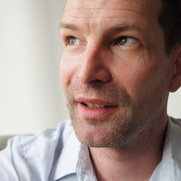
\includegraphics[width=0.3\textwidth]{images/Matthias_Schlossberger.png}
%	\caption{Matthias Schlo"sberger}
%	\label{fig:MS}
%\end{figure}


%\begin{figure}[h]
%	\centering
%	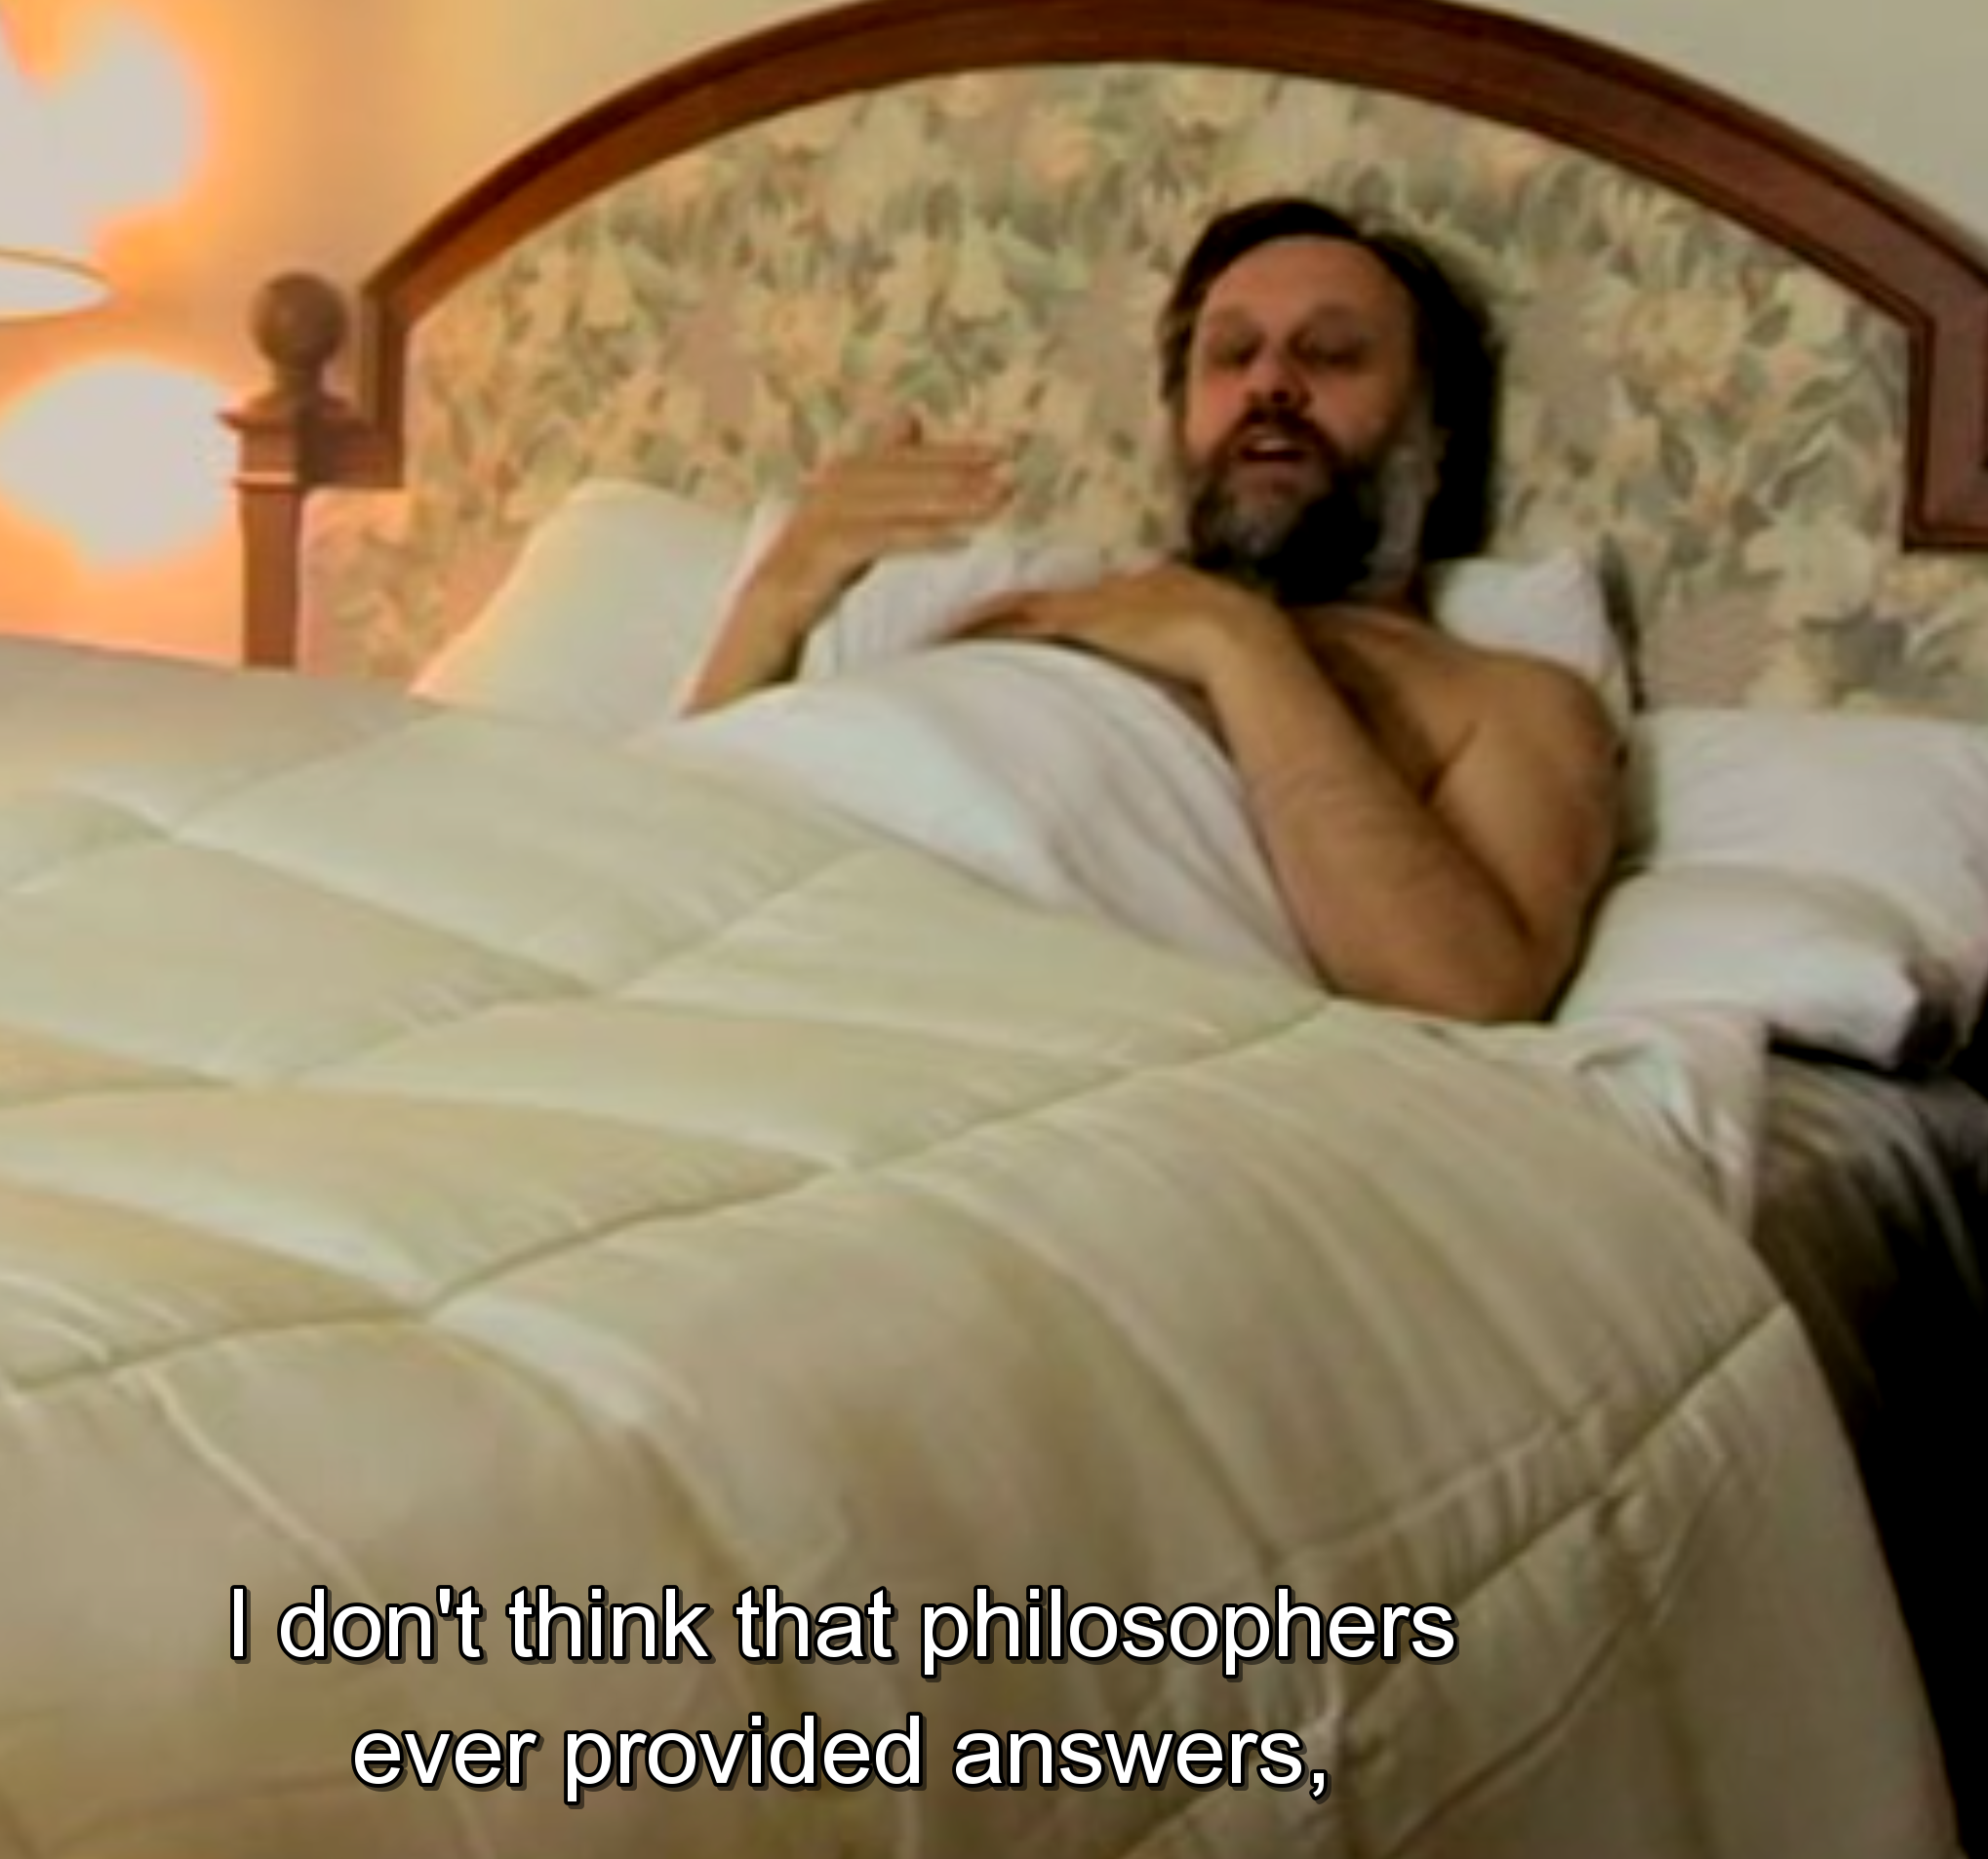
\includegraphics[width=0.5\textwidth]{images/template.png}
%	\caption{Template Bild}
%	\label{fig:template}
%\end{figure}

\end{document}
